\documentclass[11pt,psfig]{article}
\usepackage{epsfig}
\usepackage{times}
\usepackage{amssymb}
\usepackage{float}

\newcount\refno\refno=1
\def\ref{\the\refno \global\advance\refno by 1}
\def\ux{\underline{x}}
\def\uw{\underline{w}}
\def\bw{\underline{w}}
\def\ut{\underline{\theta}}
\def\umu{\underline{\mu}} 
\def\bmu{\underline{\mu}} 
\def\be{p_e^*}
\newcount\eqnumber\eqnumber=1
\def\eq{\the \eqnumber \global\advance\eqnumber by 1}
\def\eqs{\eq}
\def\eqn{\eqno(\eq)}

 \pagestyle{empty}
\def\baselinestretch{1.1}
\topmargin1in \headsep0.3in
\topmargin0in \oddsidemargin0in \textwidth6.5in \textheight8.5in
\begin{document}
\setlength{\parskip}{1.2ex plus0.3ex minus 0.3ex}


\thispagestyle{empty} \pagestyle{myheadings} \markright{Homework
1: CS 216, Image Understanding: Spring 2014}



\title{CS 216 Homework 1}
\author{Zachary DeStefano, 15247592}
\date{Due Date: April 9}

\maketitle

\vfill\eject

\section*{Problem 4}

\subsection*{Problem 4a}

The variable $x$ will be assigned to an array that is the numbers 1 through 5 arranged in a random order. 

\subsection*{Problem 4b}

The variable $a$ will be assigned to an array that is the numbers 1 through 10 arranged in chronological order. The variable $b$ will end up being assigned an array that is the numbers $1,4,7,10$ because it is the first number and then every third number after that. 

\subsection*{Problem 4c}

The variable $f$ will be assigned to an array that is the numbers 1501 to 2000 in chronological order. The variable $g$ will be assigned to the indices of $f$ where the entries are greater than $1850$ which is $351$ to $500$. The variable $h$ will then be assigned an array that is the numbers $1851$ to $2000$.  

\subsection*{Problem 4d}

The variables $x$ will be assigned to a vector of 10 entries where each entry has value 22. The variable $y$ will be assigned the sum of the entries which will be 220.

\subsection*{Problem 4e}

The variable $a$ will be assigned an array that is the numbers 1 to 1000 in chronological order. The variable $b$ will be assigned a vector that is the numbers 1 to 1000 in reverse order. 

%\begin{figure}[H]
%\centering
%\includegraphics[height=4in]{prob1plot.jpg}
%\caption{Probability of Class Labels with decision boundaries marked}
%\end{figure}

\section*{Problem 5}

\begin{figure}[H]
\centering
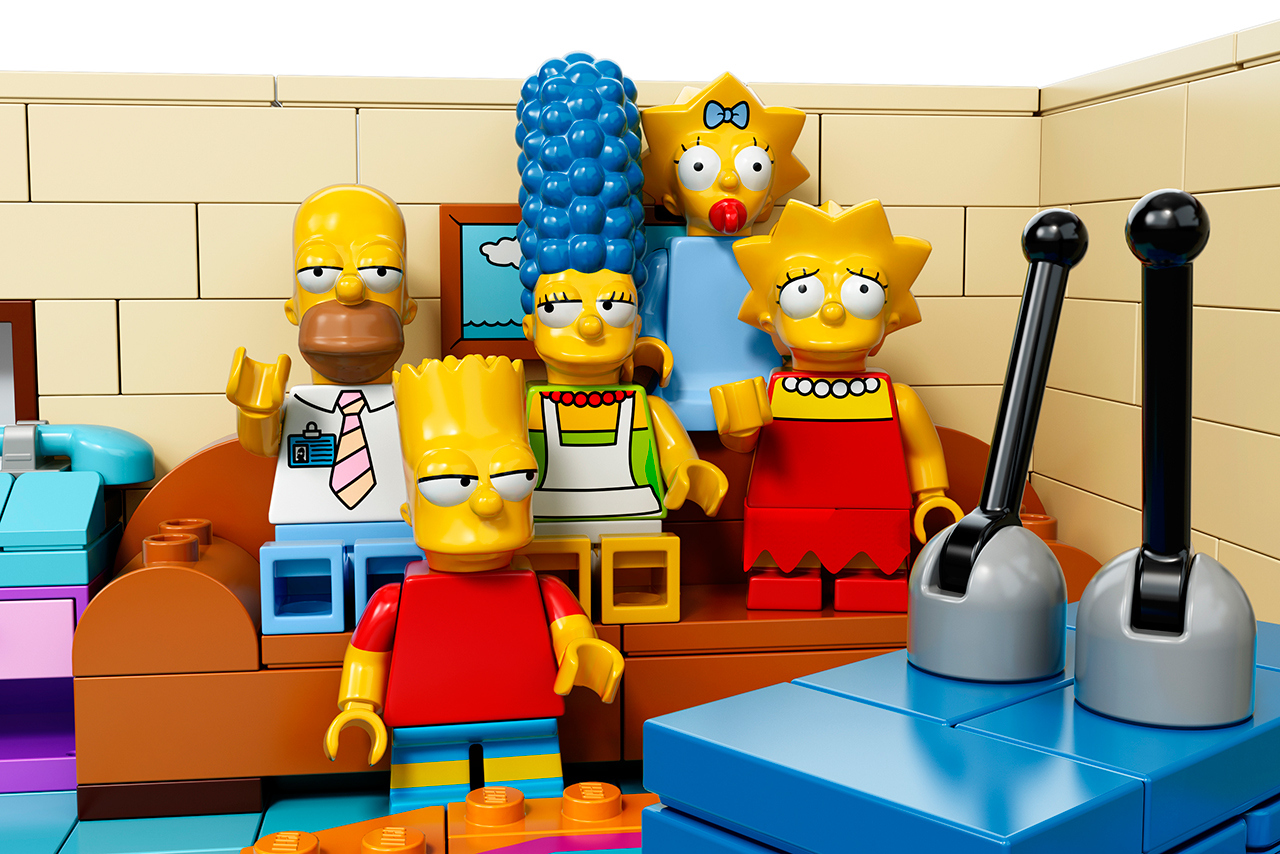
\includegraphics[height=4in]{originalImageProb5.jpg}
\caption{Original Image from the Internet}
\end{figure}

\begin{figure}[H]
\centering
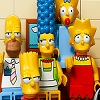
\includegraphics[height=1in]{modifiedImageProb5.jpg}
\caption{Modified 100 by 100 image}
\end{figure}

\begin{figure}[H]
\centering
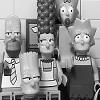
\includegraphics[height=1in]{blackWhiteImage.jpg}
\caption{Modified 100 by 100 image in grayscale}
\end{figure}

Here is the initialization code:

\begin{verbatim}

A = rgb2gray(imread('modifiedImageProb5.jpg'));
A = im2double(A);
imwrite(A,'blackWhiteImage.jpg','JPEG');

\end{verbatim}

\subsection*{Problem 5a}

\begin{figure}[H]
\centering
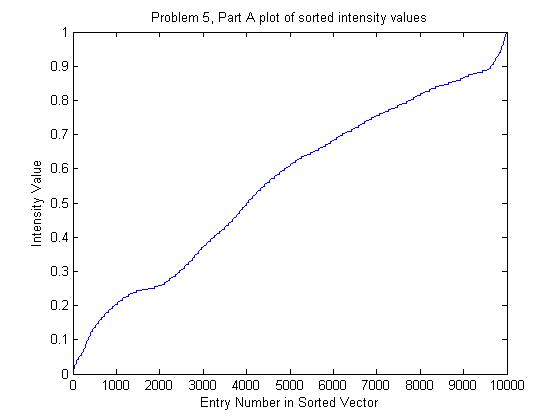
\includegraphics[height=2in]{prob5partAplot.jpg}
\caption{Plot of Intensity Values}
\end{figure}

Here is the code used to get the plot:

\begin{verbatim}

singleVectorA = A(:);
sortedValuesA = sort(singleVectorA);
figure
plot(sortedValuesA);
xlabel('Entry Number in Sorted Vector');
ylabel('Intensity Value');
title('Problem 5, Part A plot of sorted intensity values');

\end{verbatim}

\subsection*{Problem 5b}

\begin{figure}[H]
\centering
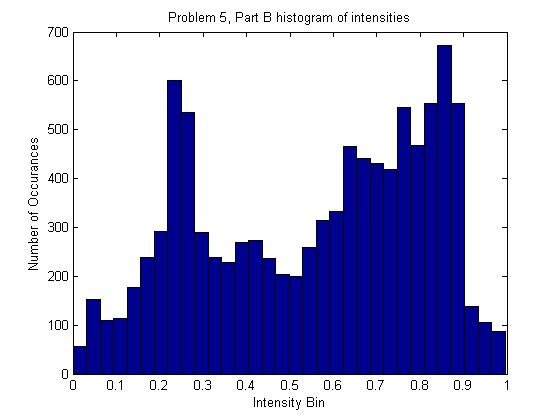
\includegraphics[height=2in]{prob5partBplot.jpg}
\caption{Histogram of Intensities with 32 bins}
\end{figure}

Here is the code used to get the plot:

\begin{verbatim}

figure
hist(singleVectorA,32);
xlabel('Intensity Bin');
ylabel('Number of Occurances');
title('Problem 5, Part B histogram of intensities');

\end{verbatim}

\subsection*{Problem 5c}

\begin{figure}[H]
\centering
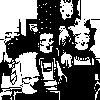
\includegraphics[height=1in]{partCimage.jpg}
\caption{Binary Image using 0.65 as the threshold}
\end{figure}

Here is the code used to get the image:

\begin{verbatim}

threshold = 0.65;
binaryA = zeros(size(A));
binaryA(A > threshold) = 1;
imwrite(binaryA,'partCimage.jpg','JPEG');

\end{verbatim}

\subsection*{Problem 5d}

\begin{figure}[H]
\centering
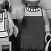
\includegraphics[height=0.5in]{partDimage.jpg}
\caption{Bottom Right Quadrant of A}
\end{figure}

Here is the code used to get the image:

\begin{verbatim}

sizeA = size(A);
sizeAhoriz = sizeA(1);
sizeAvert = sizeA(2);
bottomRightA = A(sizeAhoriz/2:sizeAhoriz,sizeAvert/2:sizeAvert);
imwrite(bottomRightA,'partDimage.jpg','JPEG');

\end{verbatim}

\subsection*{Problem 5e}

\begin{figure}[H]
\centering
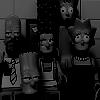
\includegraphics[height=1in]{partEimage.jpg}
\caption{New image with mean subtracted}
\end{figure}

Here is the code used to get the image:

\begin{verbatim}

meanBrightness = mean(singleVectorA);
meanSubtractedA = A-meanBrightness;
meanSubtractedA( meanSubtractedA < 0) = 0;
imwrite(meanSubtractedA,'partEimage.jpg','JPEG');

\end{verbatim}

\subsection*{Problem 5f}

\begin{verbatim}

function [ result ] = diceRoll_partF()
%DICEROLL_PARTF Summary of this function goes here
%   Detailed explanation goes here

result = floor(rand(1)*6) + 1;

end

\end{verbatim}

\subsection*{Problem 5g}

\begin{verbatim}

y = [1:6];
z = reshape(y,3,2);

\end{verbatim}

\subsection*{Problem 5h}

Result is that $x=0$ and $[r,c]=[95,99]$. Code to accomplish it is the following

\begin{verbatim}

x = min(singleVectorA);
[r,c] = find(A==x,1);

\end{verbatim}

\subsection*{Problem 5i}

The result is 5 unique values. Here is the code that was used:

\begin{verbatim}

v = [1 8 8 2 1 3 9 8];
sizeUniqueV = size(unique(v));
numUnique = sizeUniqueV(2);

\end{verbatim}

\subsection*{Problem 5 Compiled Code}

Here is the entire script used for problem 5, except for part F which was a separate function. This just puts all the code pieces from the previous sections together:

\begin{verbatim}

A = rgb2gray(imread('modifiedImageProb5.jpg'));
A = im2double(A);
imwrite(A,'blackWhiteImage.jpg','JPEG');

%Part A
singleVectorA = A(:);
sortedValuesA = sort(singleVectorA);
figure
plot(sortedValuesA);
xlabel('Entry Number in Sorted Vector');
ylabel('Intensity Value');
title('Problem 5, Part A plot of sorted intensity values');

%Part B
figure
hist(singleVectorA,32);
xlabel('Intensity Bin');
ylabel('Number of Occurances');
title('Problem 5, Part B histogram of intensities');

%Part C
threshold = 0.65;
binaryA = zeros(size(A));
binaryA(A > threshold) = 1;
imwrite(binaryA,'partCimage.jpg','JPEG');

%Part D
sizeA = size(A);
sizeAhoriz = sizeA(1);
sizeAvert = sizeA(2);
bottomRightA = A(sizeAhoriz/2:sizeAhoriz,sizeAvert/2:sizeAvert);
imwrite(bottomRightA,'partDimage.jpg','JPEG');

%Part E
meanBrightness = mean(singleVectorA);
meanSubtractedA = A-meanBrightness;
meanSubtractedA( meanSubtractedA < 0) = 0;
imwrite(meanSubtractedA,'partEimage.jpg','JPEG');

%diceRoll_partF.m is part F

%Part G
y = [1:6];
z = reshape(y,3,2);

%Part H
x = min(singleVectorA);
[r,c] = find(A==x,1);

%Part I
v = [1 8 8 2 1 3 9 8];
sizeUniqueV = size(unique(v));
numUnique = sizeUniqueV(2);

\end{verbatim}


\end{document}








